\documentclass[pdftex,12pt,letter]{article}
\usepackage{fancyhdr}
\usepackage{enumerate}
\usepackage{tabularx}
\usepackage{graphicx}
\usepackage{array}
\usepackage[justification=justified,singlelinecheck=false]{caption}
\usepackage{placeins}
\pagestyle{fancy}
\makeatletter
  \renewcommand\@seccntformat[1]{\csname the#1\endcsname.\quad}
\makeatother

\newcolumntype {Y}{ >{\raggedright \arraybackslash }X}
\newcommand{\HRule}{\rule{\linewidth}{0.5mm}}
\captionsetup{labelformat=empty}

\begin{document}

\begin{titlepage}
\begin{flushright}
\HRule \\[0.4cm]
{ \bfseries
{\huge Design Document\\[1cm]}
{\Large for\\[1cm]}
{\huge CWRUtility\large\\[4cm]}
{\large Prepared by\\Jason Kuster, Stuart Long, and William Ordiway\\[1cm]
Version 1.0 initial\\[1cm]
KOALAA Development\\[1cm]
October 6, 2012}}
\end{flushright}
\end{titlepage}
\tableofcontents{}
\begin{table}[!t]
\caption*{\bfseries Revision History}
\begin{tabularx}{\textwidth }[t]{|l|Y|Y|l|}
\hline
\bfseries Name & \bfseries Date & \bfseries Reasons for Change & \bfseries Version \\ \hline
Long & 10/6/2012 & Initial Outline & 1.0 initial\\
\hline
\end{tabularx}
\end{table}
\FloatBarrier
\newpage
\clearpage
\section{Overview}
\subsection{Overall Design}
The \emph{CWRUtility} application is essentially a collection of CWRU-related features that allows for easy, centralized access to each of the features. The complete list of features and their description can be found in the \emph{CWRUtility} SRS. Since this software system can be easily broken down into separate, uncoupled features, the design of the overall system is also broken down. Each feature will have it's own design, documented below in the "Features" section, that will operate independently of the other features. The only exception to this rule is the "StartPage" feature, which can also be seen as the overall application manager. Explained in detail below, the "StartPage" feature will be responsible for navigating the system to the different features and controlling any communication between the features. The figure below shows the various components of the system and how they are linked. This diagram could be seen as the highest level of design for the system.
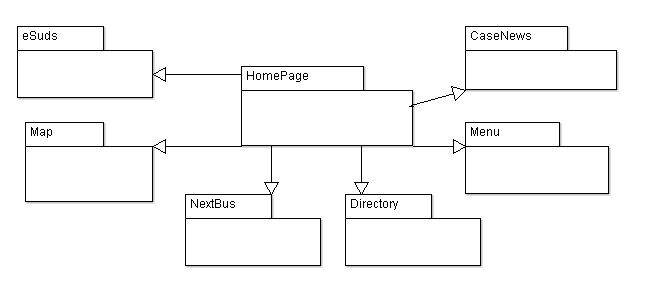
\includegraphics[width=120mm]{OverallCD.png}
\subsection{User Interface}
The implementation of any user interfaces on the Windows Phone 7/8 platform is done using the Extensible Application Markup Language (XAML). Essentially, XAML can be used as a layout language similar to HTML. It is important to note that a markup language is very dissimilar to a programming language as it works through simply creating a series of attributes and assigning values to them. The Windows Phone OS actually handles creating the UI based on these attributes, therefore this software system does not have to.
\\
\section{Features}
\subsection{Map}
The "Map" feature will allow the users to view a map of the Case Western Reserve University Campus. The feature will use the interactive map controller provided by the Windows Phone SDK. This map controller is the same map controller used for the default Windows Phone 7 map application. Since the map controller is already provided by the Windows Phone SDK, this feature will have a simple design.
\subsection{Class Diagram}
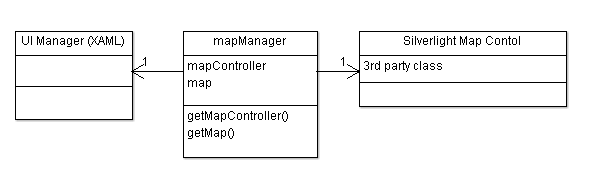
\includegraphics[width=120mm]{MapCD.png}
\subsection{Class Descriptions}
\subsubsection{SilverlightMapControl}
The SilverlightMapControl class is part of a third party library provided by Microsoft Corporation. It provides basic map controls such as zooming in, zooming out, and panning for any provided map. The MapManager will simply send a saved map of the CWRU campus to the map controller. The MapControl provides a view controller that can be placed within an application and allows the user to manipulate whatever is in its view like a map. So in this case, the view controller's view will be the map passed in by the MapManager.
\subsubsection{MapManager}
The MapManager class is responsible for overseeing the other two classes: the SilverlightMapControl and the UI manager. It will have a saved copy of the CWRU map that it will send to the SilverlightMapControl. It will also be responsible for sending the SilverlightMapControl view controller to the UI manager so that the UI manager can display the map and its view control.
\subsubsection{UIManager}
The UIManager for this feature will not be a true class, since all UI for Windows Phone is done using XAML files. Still, this manager will be responsible for laying out the components of the feature. Namely, it will have to layout the title of the application at the top, the name of this feature below that, and the actual map will take up most of the application. The XAML file will be sent the map controller (along with that map controller's view, i.e. the map)  by the MapManager.


%\subsection{Schedule}
%The "Schedule" feature will allow users to add classes or custom events to a saved schedule on the system. This feature will require three classes: a schedule event, a schedule event manager to handle schedule events, and a UI manager for the schedule.
%\subsection{Class Diagram}
%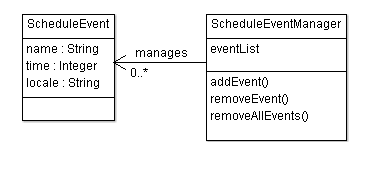
\includegraphics[width=80mm]{ScheduleEventsCD.png}
%\figurename{Schedule Class Diagram}
%\subsection{Class Descriptions}
%The following class descriptions describe the above class diagram.
%\subsubsection{ScheduleEvent}
\end{document}
